%!TeX program = xelatex
% VizDOM - Báo cáo dự án (Tiếng Việt). Biên dịch bằng XeLaTeX (xem README.md).
% Overleaf: Menu -> Settings -> Compiler -> XeLaTeX (fontspec needs XeTeX/LuaTeX).
\documentclass[11pt,a4paper]{article}

\usepackage{fontspec}
\usepackage[vietnamese]{babel}
\usepackage{microtype}
\usepackage{geometry}
\geometry{margin=2.5cm}
\usepackage{graphicx}
\usepackage{booktabs}
\usepackage{caption}
\usepackage{enumitem}
\usepackage{xcolor}
\usepackage[hidelinks]{hyperref}
\usepackage{float}

\graphicspath{{figures/}}
\newcommand{\code}[1]{\texttt{#1}}
\setlength{\parskip}{0.4em}
\setlength{\parindent}{0pt}
\setlength{\tabcolsep}{4pt}

\title{\textbf{VizDOM: Sinh cây DOM trực quan từ ảnh chụp màn hình\\
phục vụ kiểm thử tự động độc lập nền tảng}}
\author{Nguyễn Huỳnh Trí Cương\\
\small Đồ án ứng dụng thạc sĩ (Ngành Khoa học máy tính) --- Đại học Khoa học Tự nhiên TP. Hồ Chí Minh\\
\small Khoa Công nghệ thông tin\\
\small Giảng viên hướng dẫn: PGS.TS Nguyễn Văn Vũ}
\date{2026}

\begin{document}
\maketitle

\begin{abstract}
\noindent
Kiểm thử tự động giao diện đồ họa (GUI) phụ thuộc vào khả năng xác định vị trí các
phần tử trên màn hình một cách tin cậy. Cơ chế tiêu chuẩn là cây trợ năng của nền
tảng (Android UI Automator, Windows UIA, DOM của web), nhưng một lớp lớn các ứng
dụng --- giao diện desktop được vẽ tùy biến (Qt/QML, OpenGL, game engine), HMI
nhúng/công nghiệp, và màn hình quan sát qua camera --- hoàn toàn không cung cấp cây
trợ năng khả dụng, buộc người kiểm thử phải dùng các kịch bản tọa độ điểm ảnh dễ
gãy. Đồ án này trình bày \textbf{VizDOM}, một hệ thống tái dựng cây DOM tương tự UI
Automator trực tiếp từ ảnh chụp màn hình bằng cách kết hợp thị giác máy tính cổ
điển, các mô hình định vị thị giác hiện đại và một bước tinh chỉnh bằng mô hình
ngôn ngữ/thị giác nhỏ (SLM/VLM). VizDOM được tổ chức theo kiến trúc lục giác (ports
and adapters), trong đó ba cách hệ thống tương tác với ứng dụng cần kiểm thử ---
\emph{chụp} (đọc màn hình), \emph{phát hiện} (tìm phần tử) và \emph{tác động} (điều
khiển đầu vào) --- là các chiến lược cắm-thay được, có thể chạy tại chỗ hoặc dưới
dạng dịch vụ gRPC từ xa, cho phép các cấu hình khác thường như chụp màn hình vật lý
qua camera và tác động bằng cánh tay robot. Một thư viện từ khóa Robot Framework
cung cấp cây DOM đã sinh cho kiểm thử GUI thực tế. Báo cáo được nộp theo Phương
thức 3 (đồ án ứng dụng): đóng góp mang tính kỹ thuật --- kết hợp các thành phần sẵn
có thành một hệ thống hoạt động được, dễ mở rộng và triển khai --- chứ không phải
một thuật toán học máy mới.
\end{abstract}

\newpage
\tableofcontents
\newpage

% =====================================================================
\section{Giới thiệu}
% =====================================================================

\subsection{Bối cảnh bài toán}
Kiểm thử tự động GUI sống còn nhờ một khả năng: \emph{tìm} được một phần tử trên
màn hình và định địa chỉ nó một cách tin cậy qua các lần chạy. Các khung như Appium
và Selenium lấy khả năng này từ cây trợ năng của nền tảng \cite{uiautomator,appium}.
Tuy nhiên, nhiều ứng dụng thực tế không cung cấp cây khả dụng:
\begin{itemize}[leftmargin=1.4em]
  \item giao diện desktop vẽ tùy biến --- Qt/QML, OpenGL, các giao diện vẽ trên
        canvas hoặc bằng game engine --- nơi widget chỉ là điểm ảnh chứ không phải
        đối tượng trợ năng;
  \item HMI nhúng/công nghiệp và phần mềm kiosk;
  \item màn hình quan sát \emph{qua camera} hoặc card thu hình, nơi hoàn toàn không
        có giao diện phần mềm để truy vấn.
\end{itemize}
Với những mục tiêu này, đội ngũ phải quay về các kịch bản tọa độ điểm ảnh cố định,
vốn gãy ngay khi bố cục, độ phân giải hay giao diện thay đổi. Các công cụ dựa trên
ảnh như Sikuli \cite{yeh2009sikuli} so khớp ảnh mẫu nhưng không tạo ra cây phần tử
có cấu trúc và truy vấn được.

\subsection{Mục tiêu}
Tiền đề của VizDOM rất đơn giản: nếu một người kiểm thử nhìn màn hình và biết ``đó
là nút Đăng nhập'', thì một pipeline cũng nên tái dựng được cây có cấu trúc tương
đương chỉ từ điểm ảnh và trao nó cho khung kiểm thử như thể đến từ một API trợ năng.
Vì vậy các mục tiêu là:
\begin{enumerate}[leftmargin=1.6em]
  \item sinh cây DOM tương tự UI Automator (khung bao, vai trò, văn bản, nhãn, bộ
        định vị, phân cấp) từ một ảnh chụp màn hình;
  \item giữ cho bước phát hiện \emph{cắm-thay được}, để so sánh và hoán đổi các bộ
        phát hiện cổ điển và học máy;
  \item cho phép chụp, phát hiện và tác động được triển khai \emph{đúng nơi chúng
        thuộc về} (thiết bị, máy có GPU, bộ điều khiển cánh tay robot); và
  \item đưa kết quả tới một khung kiểm thử thực tế (Robot Framework).
\end{enumerate}

\subsection{Đóng góp}
Là một đồ án ứng dụng theo Phương thức 3, các đóng góp mang tính kỹ thuật:
\begin{enumerate}[leftmargin=1.6em]
  \item \textbf{Một pipeline ảnh-sang-DOM hoạt động được}, kết hợp OCR, một bộ phát
        hiện phần tử cắm-thay được (UIED cổ điển, YOLO, hoặc Microsoft OmniParser),
        các bước làm sạch dựa trên luật, và một bước tinh chỉnh tùy chọn bằng mô
        hình nhỏ (Mục~\ref{sec:impl}).
  \item \textbf{Một kiến trúc lục giác hướng dịch vụ}, trong đó chụp, phát hiện và
        tác động là các cổng bị điều khiển; mỗi cổng có thể chạy tại chỗ hoặc dưới
        dạng dịch vụ gRPC, và mỗi cổng chấp nhận plugin do người dùng cung cấp
        (Mục~\ref{sec:arch}).
  \item \textbf{Một thư viện Visual Automation cho Robot Framework} điều khiển kiểm
        thử GUI từ cây DOM đã sinh, dùng hợp đồng tọa độ chuẩn hóa để tách không
        gian phát hiện khỏi không gian thiết bị (Mục~\ref{sec:impl}).
  \item \textbf{Một khung đánh giá} và phương pháp xây dựng tập dữ liệu để đo chất
        lượng phát hiện và chất lượng DOM (Mục~\ref{sec:eval}).
\end{enumerate}

\begin{figure}[H]
  \centering
  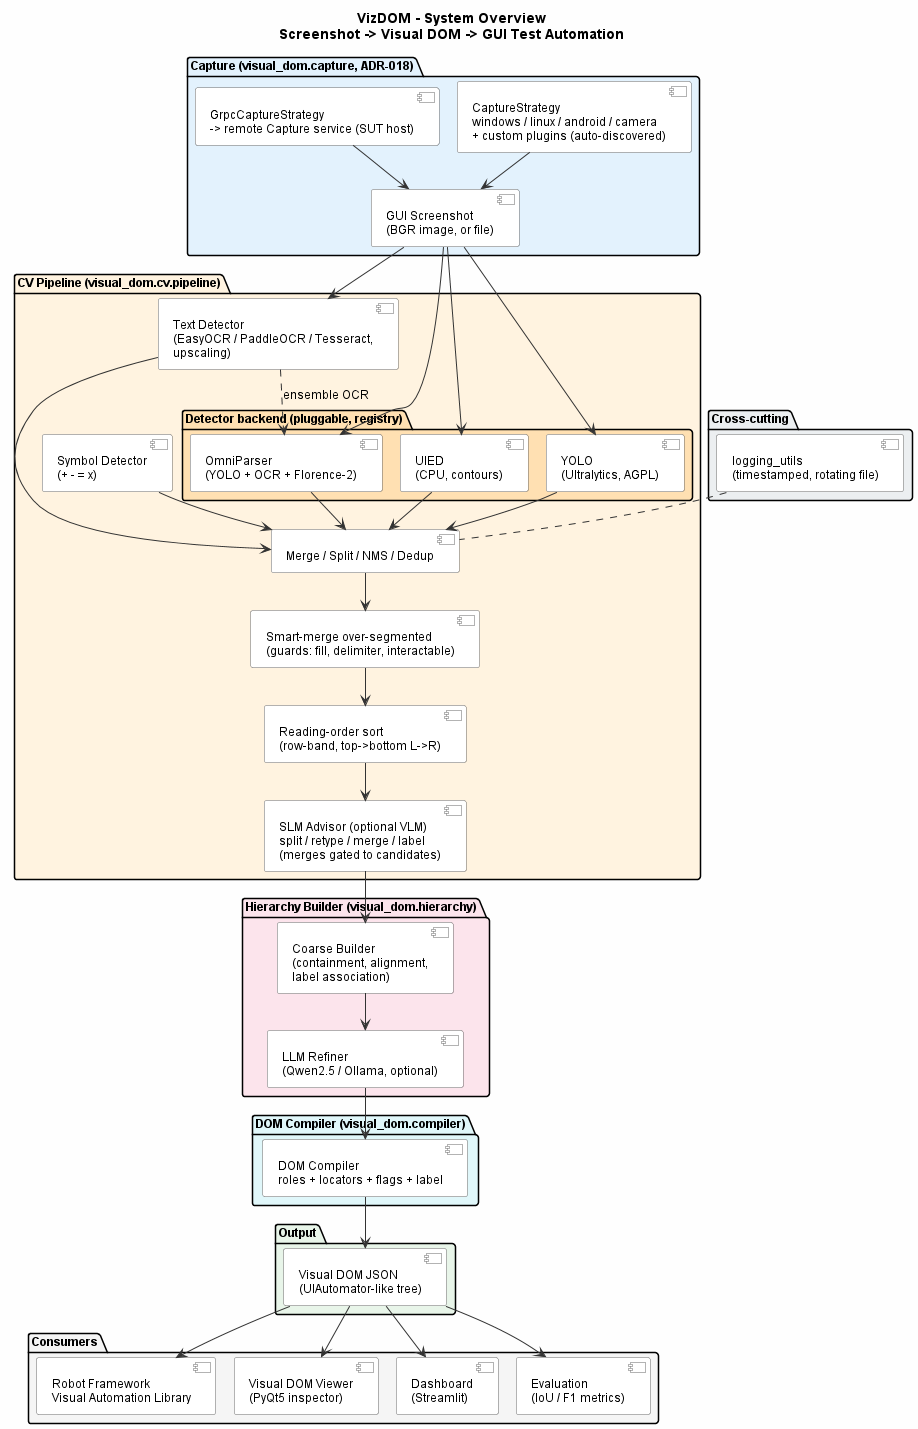
\includegraphics[width=0.62\linewidth]{System_Overview.png}
  \caption{Tổng quan hệ thống: ảnh chụp $\rightarrow$ Visual DOM $\rightarrow$ kiểm
  thử tự động. Bước chụp cấp dữ liệu cho pipeline thị giác; một bộ phát hiện
  cắm-thay được và một tầng OCR tạo ra các phần tử, sau đó được hợp nhất, sắp xếp,
  tinh chỉnh tùy chọn bằng mô hình nhỏ, dựng thành phân cấp và biên dịch thành DOM.}
  \label{fig:overview}
\end{figure}

% =====================================================================
\section{Cơ sở lý thuyết và công trình liên quan}
% =====================================================================

\subsection{Tự động hóa dựa trên trợ năng}
UI Automator, Windows UIA và DOM của web cung cấp cho khung kiểm thử một cây các
phần tử có địa chỉ \cite{uiautomator,appium}. VizDOM nhắm đúng vào các trường hợp
cây này vắng mặt hoặc không đáng tin, và \emph{tổng hợp} một cây tương đương từ điểm
ảnh.

\subsection{Tự động hóa dựa trên ảnh}
Sikuli và các công cụ tương tự \cite{yeh2009sikuli} định vị phần tử bằng so khớp
ảnh mẫu. Cách này bền vững khi thiếu dữ liệu trợ năng nhưng dễ gãy theo vị
trí/diện mạo và không cho ra phân cấp có cấu trúc, không có vai trò và không có bộ
định vị theo văn bản. VizDOM thay vào đó tạo ra cây phần tử đầy đủ.

\subsection{Phạm vi vấn đề của bài toán phát hiện phần tử GUI}
Phát hiện phần tử trong GUI không giống bài toán phát hiện đối tượng trong ảnh tự
nhiên; nghiên cứu nền tảng mà VizDOM dựa vào \cite{xie2020uied} chỉ ra các khó khăn
đặc thù của GUI ở hai cấp độ. Ở cấp \emph{phần tử}: (i) \emph{biến thiên lớn trong
cùng lớp} --- một lớp như \code{button} hay \code{input\_field} biến đổi mạnh về kích
thước, hình dạng, màu sắc và kiểu dáng theo nhà thiết kế và nội dung; và (ii)
\emph{tương đồng cao giữa các lớp} --- các lớp khác nhau có thể trông gần như giống
hệt (nút so với spinner), chỉ phân biệt bởi một dấu hiệu tinh tế như đường viền mảnh
hay một glyph nhỏ. Ở cấp \emph{GUI}: (iii) một \emph{hỗn hợp không đồng nhất} gồm
widget, hình ảnh và văn bản cùng xuất hiện và nằm sát nhau; (iv) giao diện thường
\emph{dày đặc}, các phần tử xếp sát chỉ cách nhau vài điểm ảnh; và (v) ứng dụng đòi
hỏi phát hiện \emph{vùng với độ chính xác cao} --- một hộp lỏng lẻo đủ để nhận ra một
vật trong ảnh thì không đủ để điều khiển hay khẳng định trên một điều khiển. Các đặc
điểm này trực tiếp thúc đẩy các bước làm sạch của VizDOM: hợp nhất thông minh và thứ
tự đọc (Mục~\ref{sec:impl}) tồn tại để xử lý các phần tử dày đặc, sát nhau và bị phân
mảnh, còn các hiệu ứng quy ước hộp thấy trong đánh giá (Mục~\ref{sec:eval}) là hệ quả
trực tiếp của yêu cầu độ chính xác cao. Hình~\ref{fig:problemspace} tóm tắt phân loại này.

\begin{figure}[H]
  \centering
  \includegraphics[width=0.86\linewidth]{Problem_Space.png}
  \caption{Phạm vi vấn đề của bài toán phát hiện phần tử GUI, ở cấp phần tử và cấp
  GUI (theo Xie và cộng sự~\cite{xie2020uied}). Các khó khăn này thúc đẩy các bước
  làm sạch của VizDOM và giải thích các hiệu ứng quy ước hộp trong phần đánh giá.}
  \label{fig:problemspace}
\end{figure}

\subsection{Không gian giải pháp: cổ điển, học sâu, hay kết hợp}
Với phần tử \emph{phi văn bản} có hai họ phương pháp cạnh tranh. Thị giác máy tính
\emph{cổ điển} tổng hợp cạnh/đường viền và vùng; nó không cần huấn luyện và dễ giải
thích nhưng các đặc trưng thị giác thế giới thực của nó ánh xạ kém lên các hình dạng
GUI phẳng, tổng hợp và gặp khó trên GUI có nhúng ảnh thực. Các bộ phát hiện \emph{học
sâu} hồi quy khung bao --- họ dựa trên hộp neo (Faster~R-CNN, YOLO) hoặc thiết kế
không hộp neo (CenterNet); chúng tổng quát hóa tốt nhưng nhạy cảm với định nghĩa hộp
neo, siêu tham số và dữ liệu huấn luyện, và hồi quy hộp có thể không đạt độ chính xác
GUI đòi hỏi. Phát hiện thực nghiệm của nghiên cứu nền tảng \cite{xie2020uied} là một
\emph{kết hợp} --- đề xuất vùng cổ điển cho hộp phi-văn-bản chính xác cộng một mô
hình học sâu để phân lớp, với một đường riêng cho văn bản --- vượt trội hơn từng họ
riêng lẻ. Với \emph{văn bản}, OCR có sẵn (ví dụ Tesseract) là công cụ phổ biến, nhưng
văn bản GUI khác văn bản tài liệu (nền nhiễu, gần các widget khác), nên thường cần mô
hình văn bản cảnh và xử lý riêng cho GUI.

VizDOM là một hiện thực kỹ thuật cho câu hỏi ``cổ điển, học sâu, hay kết hợp?'': cổng
phát hiện cắm-thay được khiến đường cơ sở cổ điển (UIED), các bộ phát hiện học sâu
(YOLO, OmniParser) và một lai ghép có thể chọn và so sánh trực tiếp
(Mục~\ref{sec:arch}), còn tầng OCR và tổng hợp xử lý đường văn bản. Đánh giá
(Mục~\ref{sec:eval}) chính là phép so sánh tương đương mà cách đặt vấn đề này đòi hỏi.

\subsection{Phát hiện và định vị phần tử GUI}
Phát hiện cổ điển (UIED \cite{xie2020uied}) kết hợp phân tích thành phần liên
thông/biên với OCR để tìm phần tử văn bản và phi văn bản trên giao diện sạch. Các
bộ phát hiện học máy --- họ mô hình YOLO \cite{ultralytics} và gần đây là các hệ
định vị thị giác như Microsoft OmniParser \cite{omniparser2024} (một bộ phát hiện
biểu tượng YOLO cộng mô hình chú thích Florence-2 \cite{florence2} cộng OCR) --- định
vị và mô tả các phần tử tương tác với khả năng tổng quát hóa mạnh. Các mô hình định
vị theo chỉ dẫn gần đây (Aria-UI \cite{ariaui2024}) và các bộ chuẩn định vị
(OSWorld-G/Jedi \cite{osworldg}) nhắm tới ``cho một chỉ dẫn, chỉ tới phần tử'', bổ
trợ cho mục tiêu của VizDOM là tạo ra một cây \emph{đầy đủ} thay vì một điểm định vị
đơn lẻ. VizDOM coi các bộ phát hiện này là các backend hoán đổi được thay vì cam kết
với một bộ duy nhất.

\subsection{OCR}
Văn bản được phục hồi bằng EasyOCR \cite{easyocr} và/hoặc Tesseract \cite{tesseract},
có phóng đại cho chữ nhỏ; VizDOM còn dùng OCR như một tín hiệu \emph{tổng hợp} đưa
vào OmniParser để phục hồi văn bản mà riêng bộ phát hiện bỏ sót.

\subsection{Một góc nhìn so sánh toàn cảnh}
Các hệ thống hiểu GUI gần đây chia thành hai họ. Nhóm \emph{bộ phân tích} (parser)
trả lời ``có gì trên màn hình?'' bằng cách liệt kê phần tử (UIED, OmniParser và
VizDOM); nhóm \emph{bộ định vị} (grounder) trả lời ``$X$ ở đâu?'' bằng cách trả về
một vị trí duy nhất cho một chỉ dẫn ngôn ngữ tự nhiên (Aria-UI \cite{ariaui2024},
ELAM-7B \cite{elam7b} và Jedi/OSWorld-G \cite{osworldg}). Hai họ bổ trợ nhau chứ
không thay thế nhau. Bảng~\ref{tab:models} tóm tắt các hệ thống, và
Bảng~\ref{tab:capability} đối chiếu năng lực của chúng.

\begin{table}[H]
  \centering\footnotesize
  \caption{Toàn cảnh hiểu GUI. ``n/v'' = chưa xác minh giấy phép. Các số liệu là do
  chính tác giả của mỗi hệ thống công bố.}
  \label{tab:models}
  \begin{tabular}{@{}p{2.4cm}p{2.5cm}p{2.7cm}p{0.8cm}p{2.3cm}p{2.0cm}@{}}
    \toprule
    Hệ thống & Mô hình & Độ chi tiết đầu ra & GPU & Nền tảng / kích thước & Giấy phép \\
    \midrule
    VizDOM (của ta) & parser (CV + SLM) & cây DOM phân cấp & Không$^\ast$ & pipeline ghép & tùy backend \\
    UIED & CV cổ điển & danh sách phẳng & Không & --- & nghiên cứu \\
    OmniParser V2 & phát hiện + chú thích & hộp có nhãn + khả năng tương tác & Có & YOLOv8 + Florence-2 & AGPL-3.0 / MIT \\
    Aria-UI & định vị thị giác & một điểm $[0,1000]$ & Có & Aria MoE (3.9B kích hoạt) & n/v \\
    ELAM-7B & định vị + đánh giá & điểm + PASSED/FAILED & Có & Molmo-7B-D (Qwen2-7B) & Apache-2.0 \\
    Jedi-3B/7B & định vị thị giác & một điểm & Có & 3B / 7B & n/v \\
    \bottomrule
  \end{tabular}\\[0.3em]
  {\footnotesize $^\ast$ Đường CPU qua backend UIED; backend OmniParser cần GPU để đạt tốc độ thực dụng.}
\end{table}

Hai quan sát định hình thiết kế của VizDOM. Thứ nhất, \emph{không hệ thống nào trong
bức tranh này tạo ra phân cấp}: OmniParser phát ra danh sách hộp có nhãn phẳng, còn
các bộ định vị phát ra một điểm duy nhất. Thứ hai, tất cả đều nhắm tới các
\emph{tác nhân} tự trị, vốn có yêu cầu (thành công tác vụ, tự trị) khác về bản chất
so với \emph{kiểm thử}, vốn cần tính tất định, khả lặp lại, tái sử dụng và khả chẩn
đoán.

\begin{table}[H]
  \centering\footnotesize
  \caption{Ma trận năng lực. ``Y'' = có; ``pt'' = chỉ một điểm; ``phẳng'' = danh sách phẳng.}
  \label{tab:capability}
  \begin{tabular}{@{}p{5.2cm}ccccc@{}}
    \toprule
    Năng lực & Của ta & OmniP. & Aria-UI & ELAM & Jedi \\
    \midrule
    Liệt kê mọi phần tử & Y & Y & không & không & không \\
    Phát ra khung bao & Y & Y & pt & pt & pt \\
    Cây phân cấp / DOM & Y & phẳng & không & không & không \\
    Định vị từ chỉ dẫn NL & qua DOM & không & Y & Y & Y \\
    Đánh giá đạt/không sẵn có & qua RF & không & không & Y & không \\
    Tái dùng cho nhiều hành động & Y & Y & suy lại & suy lại & suy lại \\
    Chạy không cần GPU & Y & một phần & không & không & không \\
    Đối tượng tiêu thụ & kiểm thử & tác nhân & tác nhân & kiểm thử HMI & tác nhân \\
    \bottomrule
  \end{tabular}
\end{table}

\subsection{Điểm chuẩn, và tại sao không được gộp chung}
Bảng~\ref{tab:bench} liệt kê các điểm số do tác giả công bố. Chúng đến từ
\emph{những điểm chuẩn khác nhau với độ khó khác nhau} và không được xếp chung một
bảng xếp hạng; làm vậy là sai về phương pháp. Tuy nhiên mẫu hình chung rất đáng chú
ý: định vị một bước trên các điểm chuẩn dễ gần như đã được giải (82--88\%), nhưng
trên các điểm chuẩn thực tế giảm còn 40--54\%, và thành công tác vụ đầu-cuối của tác
nhân nằm trong khoảng 15--50\%. Do đó nút thắt cổ chai không phải là độ chính xác
định vị mà là \emph{thực thi có cấu trúc, tin cậy và lặp lại được} --- chính là lập
luận cho một cây DOM tất định trong bối cảnh kiểm thử.

\begin{table}[H]
  \centering\footnotesize
  \caption{Điểm chuẩn do tác giả công bố. \textbf{Các điểm chuẩn khác nhau --- không
  so sánh trực tiếp được}; trình bày để minh họa khoảng cách dễ-so-với-thực-tế, không
  phải để xếp hạng.}
  \label{tab:bench}
  \begin{tabular}{@{}p{3.0cm}p{4.4cm}p{3.0cm}p{3.2cm}@{}}
    \toprule
    Hệ thống & Điểm chuẩn & Điểm & Ghi chú \\
    \midrule
    ELAM-7B & AutomotiveUI-Bench-4K & 87.6\% / 78.2\% & định vị / đánh giá; ô tô \\
    Aria-UI & ScreenSpot & 82.4\% & dễ, một bước \\
    Jedi-7B & OSWorld-G (564) & 54.1\% & so với UI-TARS-7B 47.5\% \\
    OmniParser V2 & ScreenSpot Pro & 39.5\% & cố tình làm khó \\
    Aria-UI & OSWorld (tác nhân) & 15.15\% & thành công tác vụ đầu-cuối \\
    Jedi-7B + o3 & OSWorld (tác nhân) & 50.2\% & so với mốc 23\% \\
    \bottomrule
  \end{tabular}
\end{table}

\subsection{Định vị VizDOM trong bức tranh}
Phát hiện phần tử nay đã là một tầng được thương mại hóa: một phòng lab công nghiệp
(OmniParser) hội tụ về cùng cách phân rã ``CV nắm hình học, mô hình thêm ngữ nghĩa'',
điều vừa xác nhận trực giác vừa loại phát hiện khỏi vai trò điểm khác biệt. Cái còn
lại thực sự đặc trưng là: (i) \emph{dựng phân cấp} --- bao hàm, căn chỉnh và liên kết
nhãn được biên dịch thành một cây truy vấn được, điều không hệ thống nào được so sánh
làm; (ii) \emph{định hướng kiểm thử} --- bộ định vị, khẳng định và từ khóa Robot
Framework; (iii) \emph{kinh tế tái sử dụng} --- một lần phân tích phục vụ nhiều bộ
định vị và khẳng định, trong khi các bộ định vị phải suy luận lại cho mỗi chỉ dẫn; và
(iv) \emph{khả giải thích} --- một cây kiểm tra được với luật so khớp truy vết được,
thay vì một tọa độ từ hộp đen. Do đó VizDOM coi các bộ phát hiện là backend hoán đổi
được, dùng bộ phát hiện mạnh nhất hiện có trong khi đóng góp nằm ở các tầng phía trên.

% =====================================================================
\section{Kiến trúc hệ thống}
\label{sec:arch}
% =====================================================================

\subsection{Cổng và bộ điều hợp theo kiến trúc lục giác}
VizDOM được tổ chức theo kiến trúc lục giác (Hình~\ref{fig:arch}). Một lõi nghiệp vụ
thuần túy, cục bộ (điều phối pipeline, logic sắp xếp và hợp nhất, dựng phân cấp thô,
biên dịch DOM) chỉ phụ thuộc vào các \emph{cổng} trừu tượng; các bộ điều hợp cụ thể
được chọn lúc chạy. Có năm cổng bị điều khiển:
\begin{itemize}[leftmargin=1.4em]
  \item \textbf{DetectorPort} --- tìm phần tử (UIED, YOLO, OmniParser, hoặc bộ phát
        hiện từ xa);
  \item \textbf{OcrPort} --- phục hồi văn bản;
  \item \textbf{RefinerPort} --- rà soát tùy chọn bằng mô hình nhỏ;
  \item \textbf{CapturePort} --- đọc màn hình; và
  \item \textbf{ActuatorPort} --- điều khiển đầu vào.
\end{itemize}
Các bộ điều hợp điều khiển (CLI, trình xem PyQt5, bảng điều khiển Streamlit và thư
viện Robot Framework) đi vào lõi qua bộ điều phối pipeline.

\begin{figure}[H]
  \centering
  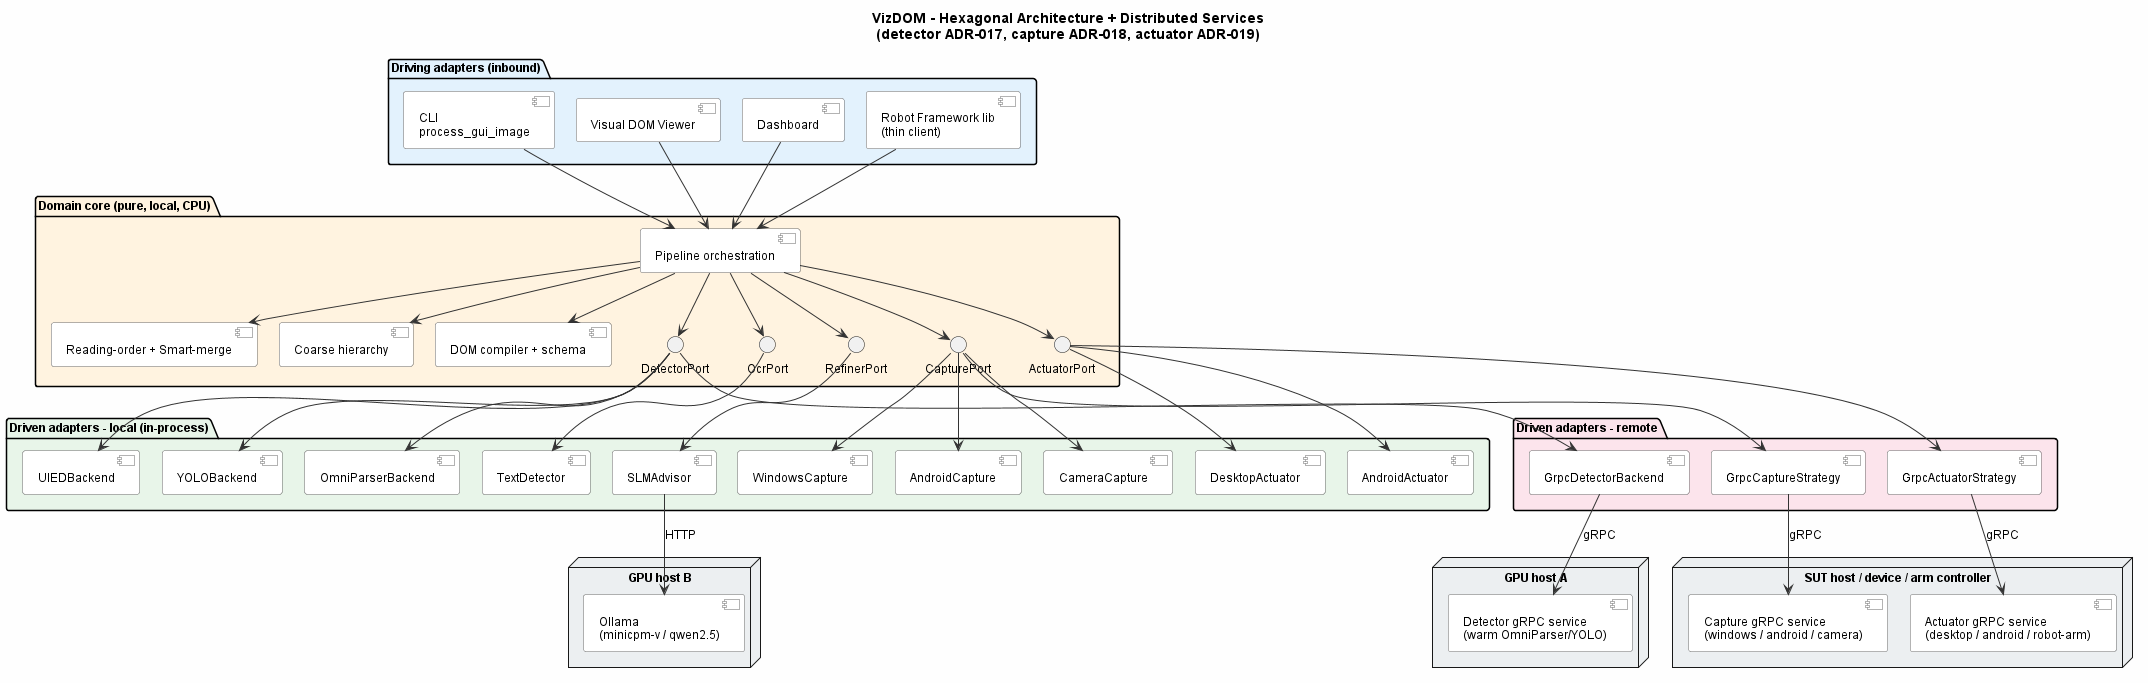
\includegraphics[width=\linewidth]{Architecture.png}
  \caption{Kiến trúc lục giác với các dịch vụ phân tán. Chụp, phát hiện và tác động
  là các cổng bị điều khiển; mỗi cổng có bộ điều hợp tại chỗ và một bộ điều hợp gRPC
  từ xa, nên các dịch vụ có thể chạy trên thiết bị cần kiểm thử, máy GPU và bộ điều
  khiển cánh tay robot tương ứng.}
  \label{fig:arch}
\end{figure}

\subsection{Chiến lược cắm-thay được và tự động khám phá}
Mỗi cổng chụp, phát hiện và tác động dùng cùng một khuôn mẫu: một lớp chiến lược cơ
sở, một registry và cơ chế \emph{tự động khám phá} các plugin người dùng đặt vào một
thư mục quy ước (ví dụ \code{plugins/capture/}, \code{plugins/actuator/}). Người dùng
thêm một nguồn chụp mới hoặc một cách tác động mới --- một camera, một card thu hình,
hay một cánh tay robot --- bằng cách viết một tệp kế thừa lớp chiến lược cơ sở;
registry nạp nó ở lần chạy kế tiếp và nó được chọn theo tên từ cấu hình. Điều này
khiến hệ thống mở rộng được mà không phải sửa lõi.

\subsection{Triển khai phân tán qua gRPC}
Vì việc chụp diễn ra nơi ứng dụng cần kiểm thử đang chạy, việc phát hiện hưởng lợi
từ GPU, và việc tác động xảy ra tại thiết bị hoặc một bộ điều khiển vật lý, mỗi cổng
còn có một bộ điều hợp từ xa được hậu thuẫn bởi một dịch vụ gRPC \cite{grpc}. Một
dịch vụ \emph{phát hiện} giữ mô hình nóng nạp mô hình nặng một lần và phục vụ nhiều
client nhẹ; một dịch vụ \emph{chụp} phục vụ ảnh từ thiết bị; một dịch vụ \emph{tác
động} thực hiện đầu vào trên thiết bị hoặc điều khiển cánh tay robot. Quan trọng là:
gRPC là một phương tiện truyền, không phải yêu cầu bắt buộc --- một lần chạy desktop
cục bộ dùng bộ điều hợp tại chỗ mà không cần máy chủ, còn chiến lược \code{grpc} chỉ
được chọn khi cổng nằm trên máy khác. Một cấu hình phân tán tiêu biểu là: \emph{chụp
trên thiết bị $\rightarrow$ phát hiện trên máy GPU $\rightarrow$ tác động trên
thiết bị/bộ điều khiển cánh tay $\rightarrow$ điều phối trên client}.

\subsection{Hợp đồng tọa độ cho tác động}
Việc phát hiện cho ra tọa độ theo điểm ảnh của ảnh, nhưng nơi một hành động rơi vào
phụ thuộc không gian riêng của bộ tác động. Do đó hợp đồng của bộ tác động dùng tọa
độ \emph{chuẩn hóa} trong $[0,1]$ cộng với kích thước ảnh nguồn; mỗi chiến lược ánh
xạ chúng về không gian thiết bị của mình: desktop nhân với độ phân giải màn hình,
thiết bị Android nhân với độ phân giải đầu vào, và plugin cánh tay robot áp dụng một
phép biến đổi homography hiệu chỉnh từ điểm ảnh sang tọa độ servo vật lý. Điều này
giữ cho bộ điều phối và giao thức mạng độc lập với độ phân giải của mọi thiết bị.

\subsection{Các quyết định kiến trúc và đánh đổi}
\paragraph{Cổng và bộ điều hợp thay vì một khối phân tầng.} Lõi nghiệp vụ chỉ phụ
thuộc vào các cổng trừu tượng, không phụ thuộc vào bộ phát hiện, nguồn chụp hay bộ
tác động cụ thể. Kiểu lục giác này được chọn vì khả kiểm thử (lõi chạy không cần
I/O) và khả thay thế (đổi backend mà không đụng logic nghiệp vụ); cái giá chấp nhận
là sự gián tiếp của một giao diện và một registry cho mỗi cổng, xứng đáng vì khả
thay thế là mục tiêu chất lượng hàng đầu của dự án.

\paragraph{Trích xuất dịch vụ tùy chọn, không phải microservices luôn chạy.} VizDOM
là một \emph{khối đơn có mô-đun} có thể trích từng cổng thành dịch vụ khi cần, chứ
không phải một hệ thống bị phân rã sẵn thành các microservices luôn chạy. Việc phân
tán được dẫn dắt bởi \emph{vị trí vật lý và tài nguyên}, không phải theo trào lưu:
chụp phải chạy nơi ứng dụng cần kiểm thử, phát hiện hưởng lợi từ GPU, và tác động xảy
ra tại thiết bị. Một lần chạy tại chỗ vẫn là mặc định, tránh khoản ``thuế'' vận hành
(triển khai, khám phá dịch vụ, xử lý lỗi cục bộ) mà một thiết kế luôn-phân-tán áp lên
trường hợp phổ biến.

\paragraph{gRPC thay vì REST hay hàng đợi thông điệp.} Các cổng từ xa dùng gRPC vì
hợp đồng protobuf có kiểu phù hợp cho một giao diện liên máy ổn định, khung nhị phân
của nó tải byte ảnh mà không phình do base64, và mô hình request/response đơn ánh xạ
trực tiếp vào ``lấy một khung hình'' / ``chạy phát hiện'' / ``thực hiện một cú chạm''.
REST+JSON sẽ phình tải trọng ảnh và mất hợp đồng có kiểu; hàng đợi thông điệp sẽ thêm
hạ tầng mà ràng buộc không-container loại trừ, và áp ngữ nghĩa bất đồng bộ lên các
thao tác vốn đồng bộ tự nhiên.

\paragraph{Mặc định chạy tại chỗ.} Đường gRPC chỉ được chọn khi một cổng nằm trên
máy khác; một lần chạy desktop cục bộ không phải trả chi phí mạng, tuần tự hóa hay
vòng đời máy chủ. Điều này giữ trường hợp đơn giản luôn đơn giản và trường hợp phân
tán vẫn khả thi với \emph{cùng một} mã nguồn, và là cơ chế cụ thể đứng sau mục tiêu
chất lượng khả triển khai.

% =====================================================================
\section{Hiện thực}
\label{sec:impl}
% =====================================================================

\subsection{Pipeline thị giác máy tính}
Phép biến đổi cốt lõi là \code{VisualDOMPipeline.process()}
(Hình~\ref{fig:pipeline}). Các bước gồm:
\begin{enumerate}[leftmargin=1.6em]
  \item \textbf{Thu nhận và chuẩn bị.} Lấy ảnh chụp (qua một chiến lược chụp hoặc từ
        tệp), tùy chọn nắn chỉnh ở ``chế độ camera'', và tính hệ số tỉ lệ theo độ
        phân giải.
  \item \textbf{Phát hiện văn bản.} Một bộ OCR (EasyOCR/PaddleOCR/Tesseract) có
        phóng đại tạo ra các phần tử văn bản.
  \item \textbf{Phát hiện phần tử.} Một backend phát hiện cắm-thay được chạy: UIED
        (phân tích đường viền trên CPU), YOLO, OmniParser (phát hiện biểu tượng YOLO
        + chú thích Florence-2 + OCR), hoặc lai ghép, tạo ra các phát hiện được
        chuẩn hóa về dạng \code{UIElement} chung.
  \item \textbf{Hợp nhất / tách / khử trùng lặp.} Văn bản và phần tử được hợp nhất
        theo bao hàm/IoU, tách theo vị trí văn bản, và giảm bớt bằng triệt tiêu
        phi cực đại theo loại và giữa các loại.
  \item \textbf{Hợp nhất thông minh phần bị phân mảnh.} Các hộp mảnh tạo nên một
        phần tử logic (nút nhiều dòng, dòng văn bản bị tách) được hợp nhất dưới các
        điều kiện bảo vệ --- ngưỡng tỉ lệ lấp đầy, kiểm tra ký tự phân tách, và luật
        ``tối đa một thành phần tương tác được'' --- để tránh gộp nhầm các điều
        khiển khác nhau.
  \item \textbf{Sắp xếp theo thứ tự đọc.} Phần tử được sắp trên-xuống, trái-phải
        bằng phương pháp phân dải theo hàng.
  \item \textbf{Rà soát tùy chọn bằng SLM/VLM.} Một mô hình nhỏ chạy qua Ollama có
        thể tách, đổi loại, hợp nhất và \emph{gán nhãn} các phần tử nghi vấn; việc
        hợp nhất bị giới hạn vào các ứng viên đã được duyệt về mặt hình học để mô
        hình không thể gộp các điều khiển không liên quan.
  \item \textbf{Phân cấp và đầu ra.} Một bộ dựng thô suy ra bao hàm, nhóm căn chỉnh
        và liên kết nhãn; bộ biên dịch DOM phát ra vai trò, cờ tương tác, nhiều bộ
        định vị và nhãn dễ đọc.
\end{enumerate}

\begin{figure}[H]
  \centering
  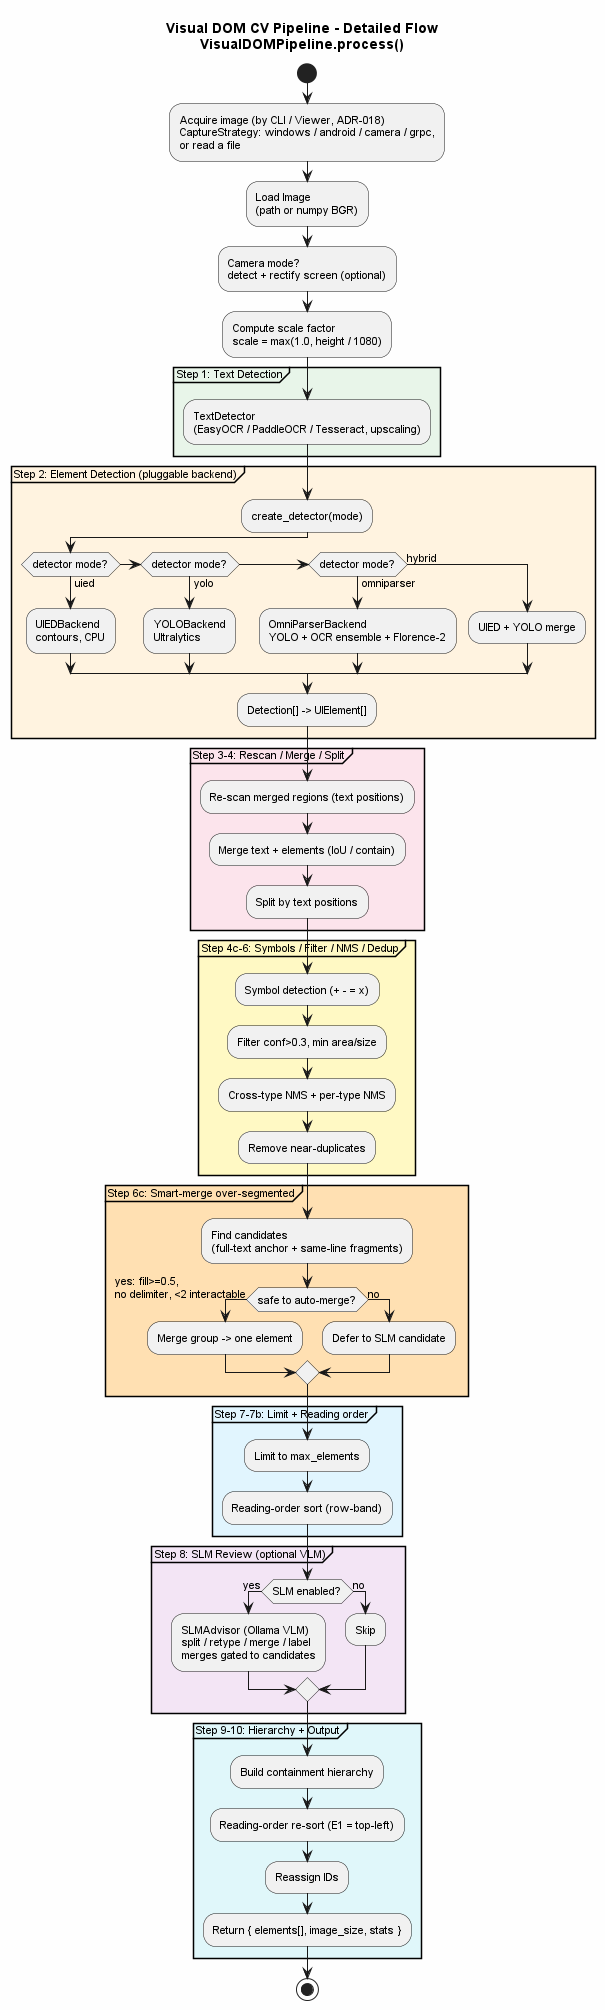
\includegraphics[height=0.86\textheight,width=\linewidth,keepaspectratio]{CV_Pipeline_Detail.png}
  \caption{Luồng điều khiển chi tiết của \code{VisualDOMPipeline.process()}: thu
  nhận, OCR, phát hiện cắm-thay được, làm sạch, hợp nhất thông minh, thứ tự đọc, rà
  soát tùy chọn bằng mô hình nhỏ, và đầu ra phân cấp/DOM.}
  \label{fig:pipeline}
\end{figure}

\subsection{Các quyết định thiết kế pipeline}
Hình dạng của pipeline xuất phát từ một số ít quyết định, mỗi quyết định là lời đáp
cho một dạng lỗi quan sát được:
\begin{itemize}[leftmargin=1.4em]
  \item \textbf{Bộ phát hiện cắm-thay được, không phải một mô hình duy nhất.} Chất
        lượng phát hiện thay đổi theo phong cách giao diện và theo phần cứng sẵn có;
        một giao diện \code{detect(image)} ổn định cho phép đường cơ sở CPU (UIED) và
        một mô hình định vị GPU (OmniParser) cùng tồn tại và được so sánh, đồng thời
        cho phép thay một bộ phát hiện AGPL bằng một bộ giấy phép dễ chịu mà không
        đụng pipeline. Đánh đổi: phải bảo trì từ hai đường mã trở lên.
  \item \textbf{Tổng hợp OCR.} Một bộ phát hiện học máy định vị tốt các phần tử tương
        tác nhưng bỏ sót chữ nhỏ; đưa một lượt OCR có phóng đại vào bộ phát hiện giúp
        phục hồi các từ bị sót (khử trùng lặp kiểu lấp khoảng trống). Đánh đổi: một
        lượt OCR thứ hai tốn thời gian, nên là tùy chọn.
  \item \textbf{Hợp nhất thông minh dựa trên luật \emph{trước} mô hình.} OmniParser
        có xu hướng phân mảnh quá mức (một nút nhiều dòng biến thành nhiều hộp). Hợp
        nhất các mảnh theo tỉ lệ lấp đầy, ký tự phân tách và luật ``tối đa một thành
        phần tương tác được'' là tất định, rẻ và giải thích được, đồng thời tránh gộp
        nhầm các điều khiển khác nhau. Đánh đổi: các ngưỡng phải chỉnh tay.
  \item \textbf{Tinh chỉnh bằng mô hình nhỏ, có kiểm soát.} Một mô hình LM/VLM nhỏ
        chỉ rà soát các phần tử nghi vấn (tách / đổi loại / hợp nhất / gán nhãn), và
        việc hợp nhất của nó bị giới hạn vào các ứng viên đã duyệt về hình học, nên
        một mô hình xác suất không bao giờ có thể gộp các điều khiển không liên quan.
        Đánh đổi: một phụ thuộc mô hình --- do đó là tùy chọn, suy giảm êm khi vắng mặt.
  \item \textbf{Hình học từ CV, ngữ nghĩa từ mô hình.} Pipeline không bao giờ để mô
        hình ngôn ngữ phát ra tọa độ; nó chỉ sở hữu nhãn và loại. Sự phân công này
        --- được xác nhận độc lập bởi thiết kế của OmniParser --- giữ độ chính xác
        không gian tất định trong khi dùng mô hình ở nơi nó mạnh.
\end{itemize}

\subsection{Các backend phát hiện cắm-thay được}
Các bộ phát hiện hiện thực một giao diện \code{DetectorBackend} chung
(\code{detect(image)} $\rightarrow$ \code{List[Detection]}, \code{is\_available()}) và được tạo bởi một
nhà máy registry. UIED là đường cơ sở CPU không phụ thuộc thư viện; YOLO và
OmniParser là các backend học máy; một backend gRPC chuyển tiếp tới dịch vụ giữ mô
hình nóng từ xa. Trên thực tế OmniParser tách các điều khiển sát nhau (ví dụ các nút
máy tính) tốt hơn UIED nhưng có xu hướng phân mảnh quá mức, điều thúc đẩy bước hợp
nhất thông minh dựa trên luật và bước tinh chỉnh có bảo vệ ở trên.

\subsection{Từ phát hiện đến DOM}
Bộ dựng phân cấp thô liên kết nhãn với điều khiển (ví dụ một trường và nhãn của nó),
nhóm các phần tử căn chỉnh và lồng theo bao hàm. Bộ biên dịch DOM sau đó tạo ra một
cây JSON tương tự UI Automator: mỗi nút mang id, khung bao, tâm, vai trò, loại trực
quan, cờ tương tác (bấm được/nhập được/cuộn được), văn bản và nhãn tùy chọn, cùng
nhiều \emph{bộ định vị} (theo id, văn bản, gợi ý, vai trò và quan hệ không gian).

\subsection{Thư viện Visual Automation cho Robot Framework}
Sản phẩm bàn giao thứ hai là một thư viện Robot Framework \cite{robotframework} đóng
vai trò một bộ điều phối mỏng trên các cổng chụp và tác động. Các từ khóa tiêu biểu:
\begin{itemize}[leftmargin=1.4em]
  \item \emph{Chụp / phân tích}: \code{Capture Screen}, \code{Dump Visual DOM},
        \code{Load Visual DOM};
  \item \emph{Truy vấn}: \code{Get Visual Element}, \code{Get Element Property},
        \code{Get Element Text}, \code{Get Element Label}, \code{Get Element Center};
  \item \emph{Hành động}: \code{Click Visual}, \code{Type Text Visual},
        \code{Press Key}, \code{Scroll Visual}, \code{Drag And Drop Visual};
  \item \emph{Khẳng định / chờ}: \code{Visual Should Exist},
        \code{Visual Should Not Exist}, \code{Wait Until Visual Appears},
        \code{Wait Until Visual Disappears}.
\end{itemize}
Bộ định vị hỗ trợ \code{id=}, \code{text=}, \code{hint=}, \code{role=} và các quan
hệ không gian (\code{within=}, \code{right\_of=}, \code{below=}, \dots). Hành động
phân giải một bộ định vị thành phần tử, chuyển tâm của nó sang tọa độ chuẩn hóa và ủy
thác cho bộ tác động, nên cùng một kịch bản chạy được tại chỗ, qua gRPC, hoặc trên
cánh tay robot mà không cần đổi. Hình~\ref{fig:seq} minh họa tương tác đầu-cuối cho
một chu trình ảnh-sang-DOM.

\begin{figure}[H]
  \centering
  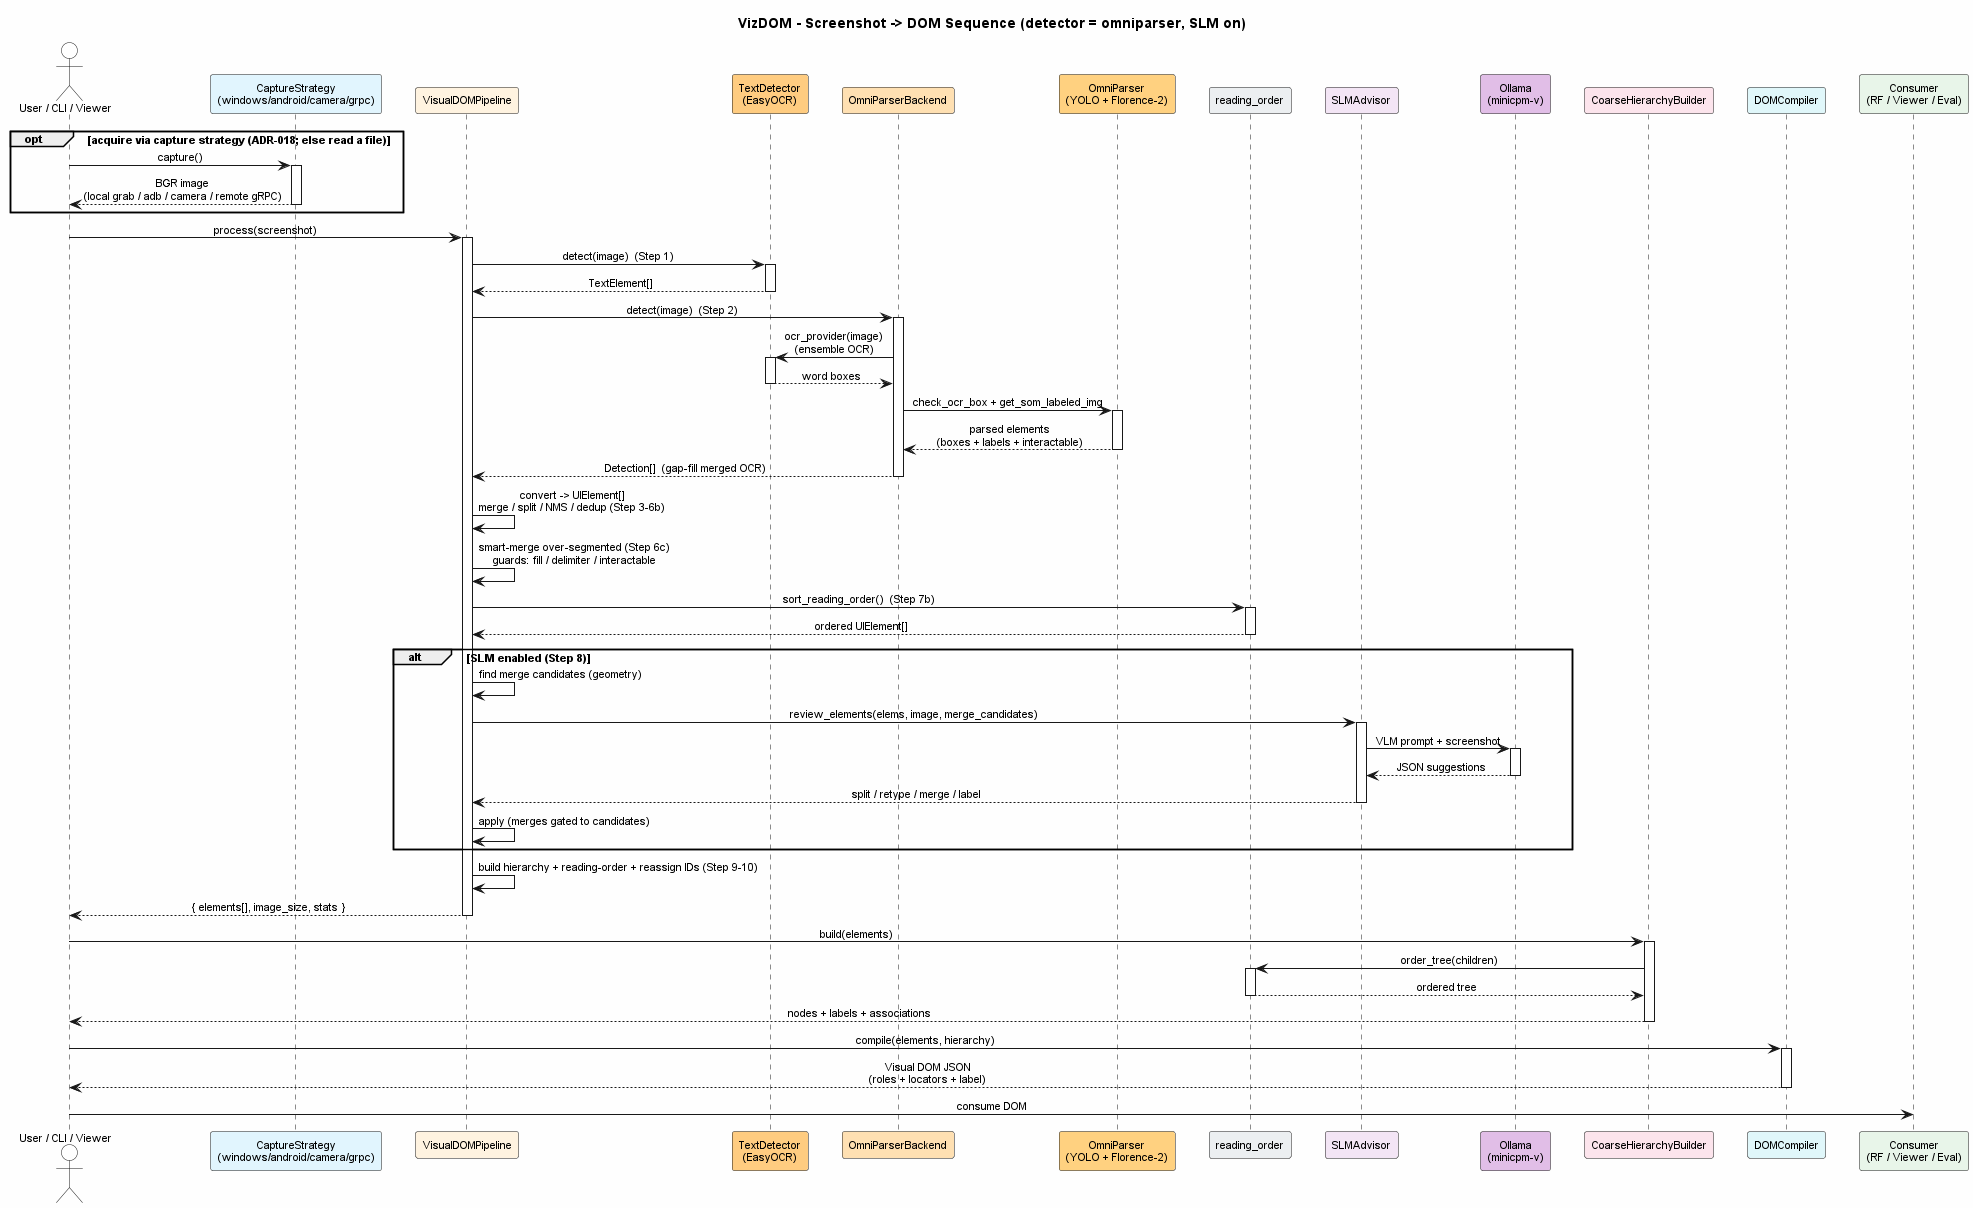
\includegraphics[width=\linewidth]{Sequence_Diagram.png}
  \caption{Trình tự một chu trình ảnh-sang-DOM (bộ phát hiện = OmniParser, bật SLM):
  chụp tùy chọn, OCR, phát hiện có tổng hợp OCR, làm sạch, thứ tự đọc, rà soát tùy
  chọn bằng mô hình nhỏ, dựng phân cấp và biên dịch DOM cho bên tiêu thụ.}
  \label{fig:seq}
\end{figure}

\subsection{Môi trường kỹ thuật}
Hệ thống chạy trên Python~3.9 với bản dựng PyTorch hỗ trợ CUDA; môi trường được quản
lý bằng \code{uv}. Việc phát triển nằm sau một proxy doanh nghiệp chặn các kho mã
nguồn công khai, điều đã định hình vài quyết định: mã mô hình bên ngoài được đóng gói
kèm và ghim phiên bản bằng một script cài đặt thay vì lấy dưới dạng submodule, và
trang tài liệu kết xuất các sơ đồ UML hoàn toàn ngoại tuyến từ một bộ kết xuất cục
bộ. Các công cụ hỗ trợ gồm một trình xem Visual DOM bằng PyQt5 (chụp, kiểm tra, xuất),
một bảng điều khiển Streamlit và một công cụ gán nhãn.

% =====================================================================
\section{Đánh giá}
\label{sec:eval}
% =====================================================================

\subsection{Phương pháp}
Chất lượng được đánh giá theo bốn trục bằng một bộ khung đánh giá:
\begin{itemize}[leftmargin=1.4em]
  \item \textbf{Phát hiện phần tử}: precision, recall, F1 và IoU trung bình so với
        các khung bao chuẩn được gán nhãn;
  \item \textbf{OCR}: tỉ lệ lỗi ký tự và lỗi từ (CER/WER);
  \item \textbf{Phân cấp}: độ đúng của bao hàm/liên kết nhãn; và
  \item \textbf{Chất lượng bộ định vị}: tính duy nhất và ổn định của các bộ định vị
        được sinh.
\end{itemize}
Điểm chuẩn là một \textbf{tập dữ liệu giao diện tổng hợp} (ảnh chụp sinh tự động ở
$1920\times1080$ với nhãn chuẩn chính xác --- khung bao phần tử, \code{visual\_type},
văn bản và bao hàm --- cùng lược đồ mà pipeline phát ra), chia thành 167 ảnh huấn
luyện và \textbf{44 ảnh kiểm thử}. Dự đoán là các phần tử pipeline sinh cho mỗi ảnh
kiểm thử; so khớp tham lam theo IoU ở ngưỡng 0.5. Vì nhãn chuẩn là danh sách phần tử
phẳng có tham chiếu cha (không phải cây lồng nhau) và không mang bộ định vị, ở đây báo
cáo trục phát hiện phần tử và OCR; trục phân cấp và bộ định vị cần nhãn chuẩn dạng
cây/có bộ định vị và để dành cho dữ liệu gán nhãn tương lai. Mọi số liệu do chính bộ
khung đánh giá của dự án (\code{visual\_dom.evaluation}) tính toán.

\subsection{Kiểm chứng chức năng}
Hệ thống đầu-cuối và các dịch vụ phân tán đã được kiểm chứng về mặt chức năng:
\begin{itemize}[leftmargin=1.4em]
  \item pipeline đầy đủ xử lý một ảnh giao diện tham chiếu và phát ra một DOM hợp lệ
        (hàng chục phần tử với vai trò, bộ định vị và nhãn);
  \item dịch vụ gRPC \textbf{phát hiện} nạp mô hình nóng một lần và trả về các phát
        hiện cho một client từ xa;
  \item dịch vụ gRPC \textbf{chụp} trả về một ảnh chụp giống hệt từng điểm ảnh cho
        client từ xa; và
  \item dịch vụ gRPC \textbf{tác động} tái tạo chính xác các hành động chuẩn hóa,
        ánh xạ chúng về tọa độ thiết bị ở phía máy chủ (đã kiểm chứng đầu-cuối bằng
        một bộ tác động ghi lại và một khối homography cánh tay robot mẫu).
\end{itemize}

\subsection{Kết quả định lượng trên điểm chuẩn tổng hợp}
Bảng~\ref{tab:results} báo cáo các chỉ số tổng thể (gộp) về phát hiện phần tử và OCR
trên 44 ảnh kiểm thử tổng hợp; Bảng~\ref{tab:pertype} phân tách recall theo loại phần
tử --- giàu thông tin hơn cho tình huống kiểm thử --- dưới hai lăng kính: chồng lấp
nghiêm ngặt (IoU $\geq 0.5$) và \emph{khả năng bấm trúng} (``center-hit'': một hộp dự
đoán có chứa tâm phần tử không, để kịch bản có thể bấm vào?).

\begin{table}[H]
  \centering
  \caption{Phát hiện phần tử và OCR tổng thể trên tập kiểm thử tổng hợp (44 ảnh,
  ngưỡng IoU 0.5, so khớp tham lam, gộp trên mọi phần tử). Cao hơn là tốt hơn.}
  \label{tab:results}
  \begin{tabular}{lccccc}
    \toprule
    Bộ phát hiện & Precision & Recall & F1 & mIoU & Đ.c.x.\ ký tự \\
    \midrule
    UIED (CPU)   & 0.39 & \textbf{0.71} & 0.51 & 0.68 & 0.92 \\
    OmniParser   & \textbf{0.56} & 0.59 & \textbf{0.58} & \textbf{0.67} & \textbf{0.95} \\
    YOLO         & \multicolumn{5}{c}{\emph{không đánh giá --- chưa có trọng số huấn luyện cho các lớp UI này}} \\
    \bottomrule
  \end{tabular}
\end{table}

\begin{table}[H]
  \centering
  \caption{Recall theo loại phần tử dưới hai lăng kính: chồng lấp nghiêm ngặt
  (IoU$\geq$0.5) và khả năng bấm trúng (hộp dự đoán chứa tâm phần tử). ``n'' = số
  lượng trong tập kiểm thử 44 ảnh. Thao tác được = nút + ô nhập + hộp kiểm + biểu tượng.}
  \label{tab:pertype}
  \begin{tabular}{lc cc cc}
    \toprule
    & & \multicolumn{2}{c}{UIED} & \multicolumn{2}{c}{OmniParser} \\
    \cmidrule(lr){3-4}\cmidrule(lr){5-6}
    Loại nhãn chuẩn & n & IoU$\geq$0.5 & center-hit & IoU$\geq$0.5 & center-hit \\
    \midrule
    button       & 183  & 0.82 & 0.96 & \textbf{1.00} & \textbf{1.00} \\
    input\_field & 135  & 0.95 & 0.99 & \textbf{0.99} & 0.99 \\
    checkbox     & 76   & \textbf{0.68} & 0.82 & 0.20 & \textbf{0.87} \\
    icon         & 36   & 0.08 & 0.28 & \textbf{0.67} & \textbf{1.00} \\
    text         & 1074 & \textbf{0.79} & \textbf{0.99} & 0.59 & 0.98 \\
    block        & 51   & 0.55 & 0.63 & 0.37 & 0.43 \\
    divider      & 145  & 0.00 & 0.10 & 0.00 & 0.21 \\
    \midrule
    thao tác được (gộp) & 430 & 0.77 & 0.89 & \textbf{0.83} & \textbf{0.97} \\
    \bottomrule
  \end{tabular}
\end{table}

Về tổng thể hai backend khá sát nhau (F1 0.51 so với 0.58), nhưng phân tách theo loại
cho thấy chúng trội ở các loại phần tử khác nhau. \textbf{OmniParser mạnh hơn trên
các điều khiển thao tác được mà kịch bản kiểm thử điều khiển}: định vị \emph{nút} hoàn
hảo (recall 1.00), \emph{ô nhập} 0.99, và \emph{biểu tượng} 0.67 (so với 0.08 của
UIED), với hộp chặt (mIoU 0.68) --- khớp với quan sát trực quan rằng hộp của nó chính
xác hơn. \textbf{UIED trội trên hộp kiểm} (IoU 0.68 so với 0.20) và recall \emph{văn
bản} (0.79 so với 0.59). Theo khả năng bấm trúng cả hai đều mạnh, và OmniParser gần
như hoàn hảo trên bộ thao tác được (gộp 0.97; nút/biểu tượng 1.00, ô nhập 0.99) so với
0.89 của UIED. IoU hộp kiểm thấp (0.20) nhưng center-hit cao (0.87) của OmniParser
chính là hiệu ứng quy ước hộp --- nó bao dấu tích thay vì toàn bộ điều khiển có đệm ---
nên phần tử vẫn bấm trúng được dù chồng lấp nghiêm ngặt thấp.

Hai điểm khép lại vòng lặp với quan sát định tính. Thứ nhất, điểm yếu trước đây về
\emph{phân loại} (OmniParser gán mọi thứ thành \code{text}/\code{icon}) đã được xử lý:
backend nay suy ra \code{button} / \code{input\_field} / \code{checkbox} /
\code{icon} từ tính tương tác và hình học nhận biết độ phân giải, nên DOM của nó dùng
được trực tiếp bởi tầng kiểm thử. Thứ hai, với tình huống kiểm thử GUI --- nơi một
phần tử chủ yếu cần \emph{bấm trúng} tin cậy --- OmniParser là lựa chọn mặc định mạnh
hơn trên điểm chuẩn này, còn UIED vẫn là đường cơ sở không cần GPU và là lựa chọn tốt
hơn nơi recall văn bản hoặc hộp kiểm chiếm ưu thế. Lưu ý: đây là tập \emph{tổng hợp,
sạch} (điểm tuyệt đối sẽ khác trên giao diện thực tế); tổng hợp OCR không tạo thay đổi
đo được ở đây (OCR sẵn có của OmniParser đã bắt hết văn bản); và biến thể tinh chỉnh
bằng SLM không được đo (cần một dịch vụ Ollama đang chạy).

\subsection{Cải thiện phân loại loại phần tử của OmniParser}
Đánh giá và kiểm tra trực quan làm lộ một hạn chế độc lập với chất lượng hộp: dù
\emph{hộp} của OmniParser chính xác, tích hợp ban đầu chỉ ánh xạ mọi phát hiện thành
\code{text} hoặc \code{icon}, nên DOM không mang vai trò \code{button} /
\code{input\_field} / \code{checkbox} --- độ chính xác phân loại loại trên các điều
khiển thao tác được là \textbf{0\%} theo cấu trúc, và logic kiểm thử dựa trên vai trò
không dùng được DOM của OmniParser.

Ánh xạ cải tiến (\code{\_infer\_visual\_type}) kết hợp ba tín hiệu. Thứ nhất,
\emph{hình học}: hộp rộng cao bằng ô nhập là ô nhập, và hộp nhỏ hình vuông là một
biểu tượng điều khiển. Thứ hai, \emph{độ rộng/tỉ lệ} tách nút khỏi biểu tượng --- nút
rộng hơn hẳn (độ rộng trung vị đo được $\approx 2\times$ biểu tượng), nên hộp rộng có
nhãn là nút còn hộp nhỏ gần vuông là biểu tượng. Thứ ba, \emph{chú thích} của
OmniParser phân biệt hộp kiểm với biểu tượng (cả hai đều là ô vuông nhỏ): chú thích
chứa ``check'', ``toggle'', ``radio'' hay ``switch'' đánh dấu một hộp kiểm. Ngoài ra,
pipeline nay tự phân giải đường dẫn mô hình OmniParser, vì đường dẫn thiếu trước đây
đã âm thầm làm một lần chạy suy giảm về chỉ-OCR.

Bảng~\ref{tab:typeacc} cho thấy hiệu quả qua hai giai đoạn đo được. Ánh xạ ban đầu
chỉ đạt độ chính xác loại thao tác được 0.09 --- đúng duy nhất trên biểu tượng, mà nó
có được một cách tầm thường do gán \emph{mọi thứ} thành \code{icon}. Một \emph{sửa lần
đầu} thêm suy luận vai trò dựa trên tính tương tác và hình học (chiều cao ô nhập và
rộng/tỉ lệ), giúp hồi phục nút (0.91) và ô nhập (0.99) và nâng độ chính xác thao tác
được lên 0.73 --- nhưng nó \emph{làm giảm} biểu tượng: luật hình học nay phân loại nhầm
các ô vuông nhỏ thành nút hoặc hộp kiểm, kéo độ chính xác biểu tượng từ mức 1.00 tầm
thường xuống 0.00, còn hộp kiểm gần như bằng 0 (0.12) vì không thể phân biệt hình học
với biểu tượng. Thêm \emph{chú thích} của OmniParser để phân biệt hộp kiểm, cùng việc
tinh chỉnh lại ranh giới rộng/tỉ lệ giữa nút và biểu tượng, tạo ra ánh xạ hiện tại:
biểu tượng hồi phục lên 0.89, hộp kiểm lên 0.55, nút giữ ở 0.89, và độ chính xác thao
tác được đạt \textbf{0.87}. DOM của OmniParser nay dùng được trực tiếp bởi tầng kiểm
thử trên mọi vai trò tương tác.

\begin{table}[H]
  \centering
  \caption{Độ chính xác phân loại loại trên các điều khiển thao tác được khớp, qua hai
  giai đoạn cải tiến (OmniParser, tập kiểm thử tổng hợp): \emph{trước} (chỉ text/icon),
  \emph{sửa lần đầu} (tính tương tác + hình học), và \emph{hiện tại} (+ phân biệt bằng
  chú thích và tinh chỉnh rộng/tỉ lệ). Định vị (Bảng~\ref{tab:pertype}) không đổi ---
  bảng này chỉ đo \emph{loại}. $^\dagger$Ánh xạ cũ gán mọi thứ phi-văn-bản thành
  \code{icon}, nên biểu tượng đúng một cách tầm thường còn mọi vai trò khác bằng 0.}
  \label{tab:typeacc}
  \begin{tabular}{lccc}
    \toprule
    Loại (GT) & Trước & Sửa lần đầu & Hiện tại \\
    \midrule
    button       & 0.00 & 0.91 & 0.89 \\
    input\_field & 0.00 & 0.99 & 0.99 \\
    checkbox     & 0.00 & 0.12 & 0.55 \\
    icon         & 1.00$^\dagger$ & 0.00 & \textbf{0.89} \\
    \midrule
    thao tác được & 0.09 & 0.73 & \textbf{0.87} \\
    \bottomrule
  \end{tabular}
\end{table}

Hộp kiểm vẫn là vai trò yếu nhất (0.55): chỉ hồi phục được khi chú thích của
OmniParser đủ đặc trưng (``Checkmark'', ``Toggle''), còn nhiều hộp kiểm mang chú
thích chung chung hoặc nhãn hiển thị của chúng. Dùng nhãn văn bản kế bên hoặc ngữ
nghĩa chú thích phong phú hơn để nhận diện hộp kiểm là công việc tương lai.

\subsection{Cân nhắc về hiệu năng}
Hiệu năng được phân tích theo ba trục. Các số liệu thời gian thực còn chờ điểm chuẩn
tương đương (Bảng~\ref{tab:results}), nên phần thảo luận ở đây mang tính cấu trúc và
dựa trên các đặc trưng mô hình đã công bố thay vì các số đo chưa có.

\paragraph{Dấu chân phần cứng.} Các mô hình định vị lớn và phụ thuộc GPU --- Aria-UI
kích hoạt 3.9B tham số, còn ELAM-7B và Jedi-7B thuộc lớp 7B --- trong khi backend
UIED của VizDOM chỉ dùng CPU. Một đường CPU là điểm khác biệt thực sự cho các dàn máy
kiểm thử và các thiết bị nhúng không có GPU; backend OmniParser chính xác nhưng nặng
được cung cấp cho các máy có GPU.

\paragraph{Kinh tế tái sử dụng.} Một bộ phân tích khấu hao chi phí: một lần phân tích
DOM phục vụ nhiều lượt tra cứu bộ định vị và khẳng định (khối lượng công việc mô hình
$O(1)$ theo sau bởi $n$ truy vấn cây rẻ), trong khi một bộ định vị phải suy luận lại
cho mỗi chỉ dẫn ($n$ lần gọi mô hình). Trong một bộ kiểm thử hồi quy gồm hàng nghìn
bước, khác biệt tiệm cận này là ranh giới giữa một công cụ dùng được và không dùng
được --- một lập luận hiệu năng có tính quyết định cho trừu tượng DOM trong kiểm thử,
độc lập với bất kỳ con số độ trễ đơn lẻ nào.

\paragraph{Dịch vụ giữ mô hình nóng và giảm tải.} Dịch vụ phát hiện nạp mô hình một
lần và phục vụ các yêu cầu sau đó chỉ bằng suy luận, và một máy GPU có thể phục vụ cả
một đội client CPU nhẹ. Đặt việc chụp tại thiết bị, suy luận trên máy GPU và điều
phối trên client giúp mỗi nút làm đúng việc hợp với nó, tránh phải chuyển một mô hình
nặng tới mọi máy. Điểm chuẩn dự kiến sẽ báo cáo độ trễ CPU-so-với-GPU và thông lượng
bộ phát hiện theo phương pháp ở trên.

% =====================================================================
\section{Thảo luận và hạn chế}
% =====================================================================
\begin{itemize}[leftmargin=1.4em]
  \item \textbf{Độ bền trên giao diện thực tế.} Phát hiện và nhận dạng ký hiệu mạnh
        trên giao diện sạch và tổng hợp nhưng yếu hơn trên các ứng dụng nhiều dải màu
        và giao diện tùy biến; việc giảm phân mảnh quá mức đang được tiếp tục.
  \item \textbf{Đánh giá định lượng.} Kết quả được báo cáo trên một điểm chuẩn tổng
        hợp (Mục~\ref{sec:eval}); vẫn cần một tập gán nhãn \emph{thực tế} lớn hơn để
        xác nhận các con số chuyển giao được ra ngoài giao diện sạch, và để đo được
        các trục phân cấp và bộ định vị mà nhãn chuẩn hiện tại chưa cho phép.
  \item \textbf{Hiệu chỉnh cho tác động vật lý.} Trường hợp cánh tay robot cần một
        phép hiệu chỉnh ảnh-sang-vật-lý cho mỗi thiết lập; kiến trúc cô lập việc này
        vào plugin, nhưng đây vẫn là công việc thực sự, và tác động vật lý kèm theo
        các nghĩa vụ an toàn (giới hạn vùng làm việc, nút dừng khẩn) mà plugin phải
        thực thi.
  \item \textbf{An toàn của khả năng mở rộng.} Tự động khám phá plugin nạp mã người
        dùng và các kênh gRPC hiện chưa xác thực; cả hai chấp nhận được cho dùng tin
        cậy/mạng LAN và đã được ghi nhận để gia cố (khám phá theo entry-point, TLS).
\end{itemize}

% =====================================================================
\section{Kết luận và hướng phát triển}
% =====================================================================
VizDOM cho thấy rằng có thể tái dựng một cây DOM khả dụng, tương tự UI Automator, từ
một ảnh chụp màn hình bằng cách kết hợp thị giác máy tính cổ điển, một mô hình định vị
thị giác hiện đại và một bước tinh chỉnh bằng mô hình nhỏ, và rằng engine thu được có
thể triển khai linh hoạt qua một kiến trúc lục giác hướng dịch vụ. Hệ thống đã mang
lại giá trị cho một khung kiểm thử thực tế và hỗ trợ các cấu hình khác thường như
chụp bằng camera kèm tác động bằng cánh tay robot. Hướng phát triển gồm: hoàn tất bộ
chuẩn định lượng trên một tập dữ liệu gán nhãn lớn hơn; giảm phân mảnh quá mức trên
các giao diện thực tế tùy biến; đánh giá các mô hình định vị theo chỉ dẫn (Aria-UI,
ELAM-7B, Jedi) như phương án thay thế hoặc bổ trợ cho bước tinh chỉnh bằng mô hình
nhỏ; và gia cố các dịch vụ bằng xác thực/TLS cùng cơ chế khám phá plugin theo
entry-point.

\bibliographystyle{plain}
\bibliography{references}

\end{document}
